\documentclass[preview]{standalone}
\usepackage{tkz-graph}
\begin{document}

\begin{figure}[ht]
\center
 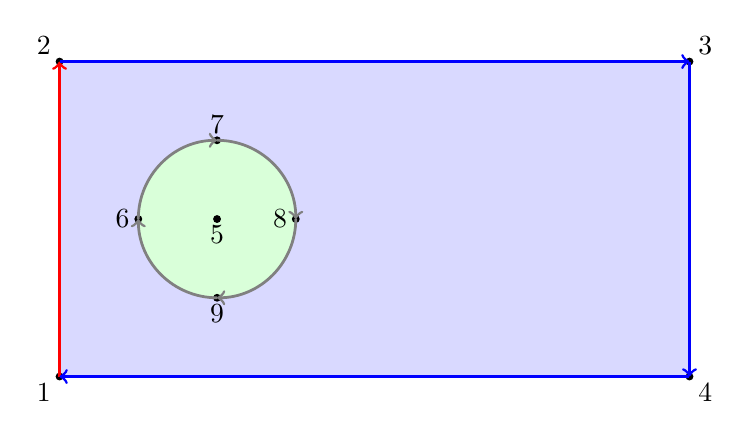
\begin{tikzpicture}
   \draw(-0.2,-0.2) node {$1$};   
   \draw(-0.2,4.2) node {$2$};   
   \draw(8.2,4.2) node {$3$};   
   \draw(8.2,-0.2) node {$4$};    
 
   \fill [blue!15] (0,0) rectangle +(8.,4.);   
   \fill [green!15] (2,2) circle (1);
 
   \fill [black] (0,0) circle (0.05); 
   \fill [black] (0,4) circle (0.05); 
   \fill [black] (8,4) circle (0.05); 
   \fill [black] (8,0) circle (0.05); 

   \draw[->,color=red,line width=1pt] (0,0) -- (0,4);
   \draw[->,color=blue,line width=1pt] (0,4) -- (8,4);
   \draw[->,color=blue,line width=1pt] (8,4) -- (8,0);
   \draw[->,color=blue,line width=1pt] (8,0) -- (0,0);

   \fill [black] (2,2) circle (0.05); 
   \draw(2,1.8) node {$5$};   
   \fill [black] (1,2) circle (0.05); 
   \draw(0.8,2) node {$6$};  
   \fill [black] (2,3) circle (0.05); 
   \draw(2,3.2) node {$7$};  
   \fill [black] (3,2) circle (0.05); 
   \draw(2.8,2) node {$8$};  
   \fill [black] (2,1) circle (0.05); 
   \draw(2,0.8) node {$9$};  

  \draw[->,color=black!50,line width=1pt]   (1,2) arc(180:90:1);
  \draw[->,color=black!50,line width=1pt]   (2,3) arc(90:0:1);
  \draw[->,color=black!50,line width=1pt]   (3,2) arc(0:-90:1);
  \draw[->,color=black!50,line width=1pt]   (2,1) arc(-90:-180:1);
 \end{tikzpicture}
\end{figure}


\end{document}



После: convert pdf to png
https://convertio.co/pdf-png/



 






